\documentclass[12pt,a4paper]{article}
\usepackage[left=2.5cm,right=2cm,top=2cm,bottom=2cm]{geometry}
\usepackage{tabularx}
\usepackage{setspace}
\usepackage{graphicx}
\usepackage{array}
\usepackage{fancyhdr}
\usepackage{times}


\pagestyle{fancy}
\renewcommand{\headrulewidth}{0pt}
\fancyhf{}
\rfoot{\thepage}

\setlength{\parindent}{0pt}
\renewcommand{\arraystretch}{1.25}

\begin{document}

\begin{center}
{\Large \textbf{RIWAYAT HIDUP}}
\end{center}

\vspace{0.5cm}

%==============================%
% BIODATA DIRI
%==============================%
\textbf{BIODATA DIRI}
\vspace{0.2cm}
\hrule
\vspace{0.5cm}

\noindent
\begin{minipage}{0.70\textwidth}
\begin{tabularx}{\textwidth}{p{3.8cm} l X}
Binusian ID         & : & 2502124914 \\
Nama                & : & Denny Chrisnanda \\
Tempat/Tanggal Lahir & : & Kediri / 12 Februari 1999 \\
Jenis Kelamin       & : & Laki-laki \\
Email               & : & denny.chrisnanda@binus.ac.id \\
\end{tabularx}
\end{minipage}
\hfill
\begin{minipage}{0.28\textwidth}
\begin{center}
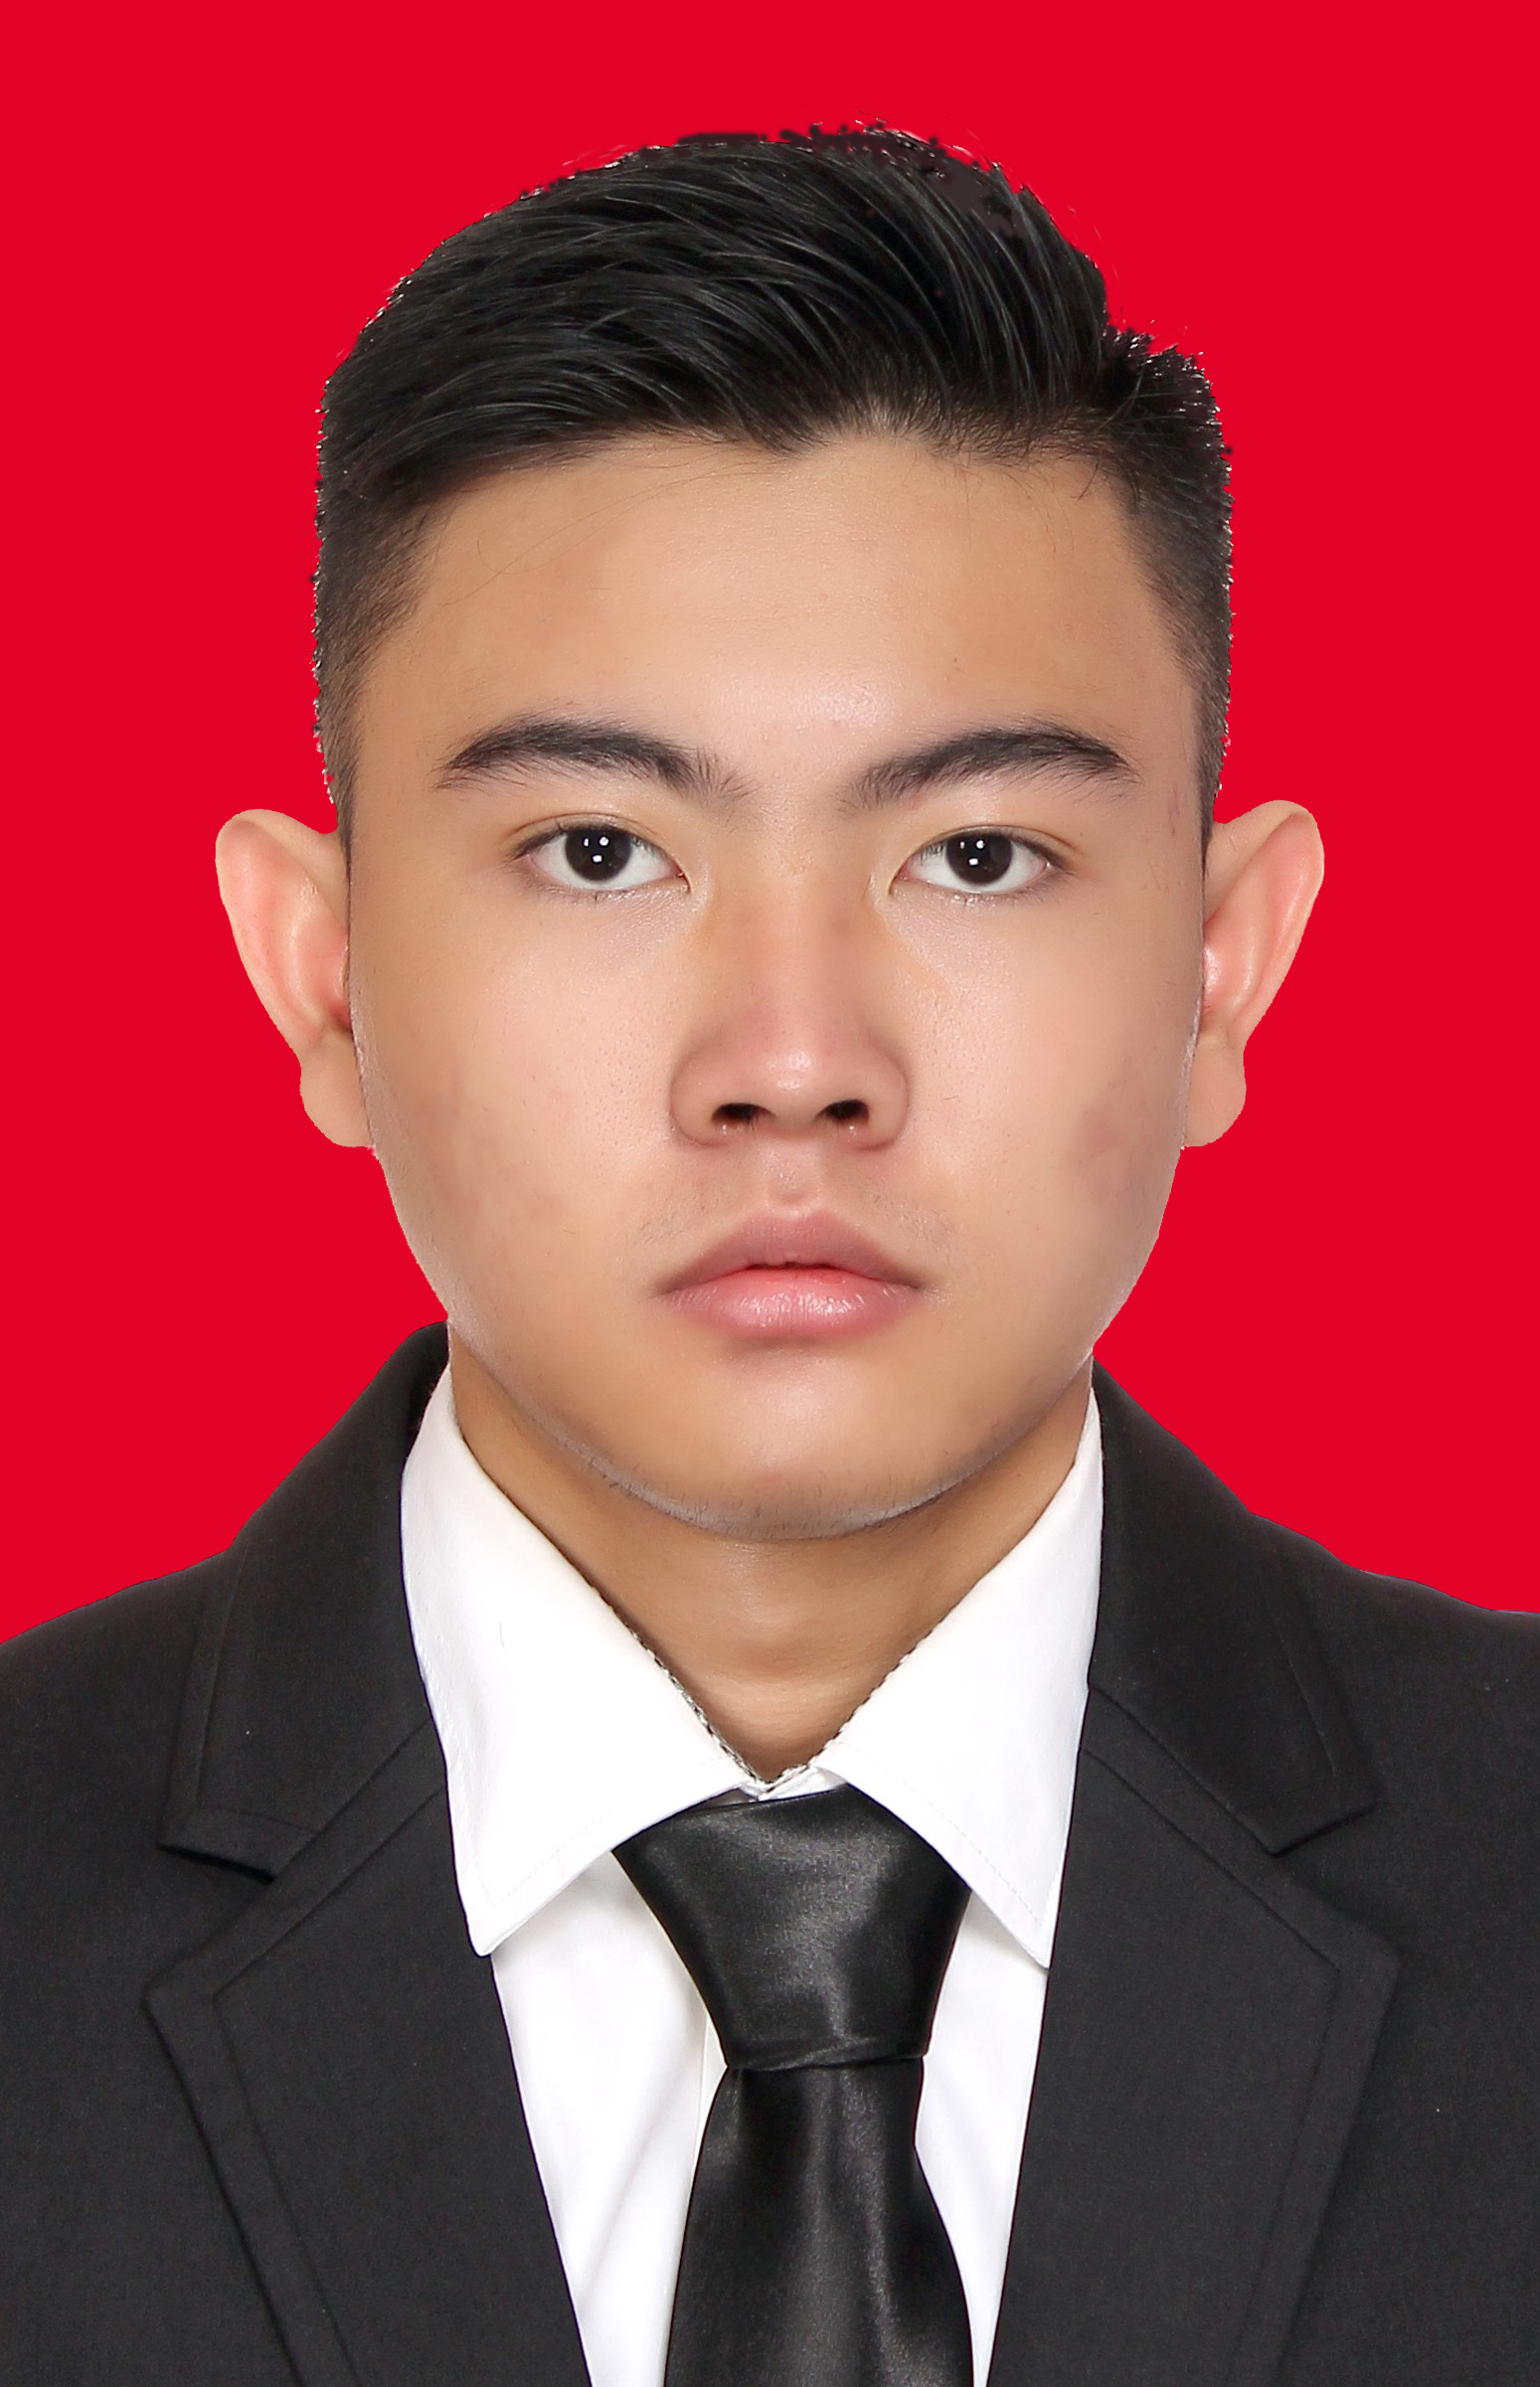
\includegraphics[width=3cm]{Graduation Photo.jpg}
\end{center}
\end{minipage}

%---- Alamat dan data lanjutan tanpa foto mengganggu ----%
\vspace{0.4cm}

\begin{tabularx}{\textwidth}{p{3.8cm} l X}
Alamat              & : &
\textbf{Domisili:} Jl Cendrawasih Blok E-48 Komplek Auri Jaladhapura .Margahayu.Bekasi Timur 17113 \\
& &
\textbf{Permanen:} RT 01 / RW 01, Dusun Pakisaji, Desa Duwet, Kecamatan Wates, Kabupaten Kediri, Jawa Timur, 64174 \\
No. HP              & : & 085645184121 \\
Kewarganegaraan     & : & Indonesia \\
Status Perkawinan   & : & Belum Kawin \\
Agama               & : & Kristen \\
\end{tabularx}

\vspace{0.8cm}
%==============================%
% RIWAYAT PENDIDIKAN
%==============================%
\textbf{RIWAYAT PENDIDIKAN}
\vspace{0.2cm}
\hrule
\vspace{0.5cm}

\textbf{Pendidikan Saat Ini}
\begin{tabbing}
\hspace{4cm} \= \hspace{10cm} \kill
Pendidikan Saat Ini \> : Strata 1 \\
Nama Sekolah \> : Universitas Bina Nusantara \\
Jurusan \> : S1 Teknik Informatika \\
Periode \> : 2022 - sekarang \\
GPA (sementara) \> : 3.87 / 4 \\
\end{tabbing}

\vspace{0.3cm}

\textbf{Pendidikan Terakhir}
\begin{tabbing}
\hspace{4cm} \= \hspace{10cm} \kill
Pendidikan Terakhir \> : SMK \\
Nama Sekolah \> : SMK Negeri 1 Kediri  \\
Jurusan \> : Teknik Otomasi Industri \\
Periode \> : 2014 - 2017 \\
%GPA \> : 3.58 / 4 \\
\end{tabbing}


%==============================%
% PENGALAMAN ORGANISASI
%==============================%
% \vspace{0.5cm}
% \textbf{PENGALAMAN ORGANISASI}
% \vspace{0.2cm}
% \hrule
% \vspace{0.4cm}

% \textbf{Himpunan Mahasiswa Mekatronika Otomasi (HIMAMO) / 2016–2019} \\
% Anggota Bidang Kaderisasi (2017–2019) \\
% Periode keanggotaan: 2016–2019

% \vspace{0.3cm}

% \textbf{Unit Kegiatan Mahasiswa Seni Budaya Minangkabau (UKM-SBM) / 2016–2019} \\
% Anggota Seni Randai (2016–2018) \\
% Ketua UKM–SBM (2018–2019) \\
% Periode keanggotaan: 2016–2019

%==============================%
% SERTIFIKASI PERSONAL
%==============================%
\vspace{0.5cm}
\textbf{SERTIFIKASI PERSONAL}
\vspace{0.2cm}
\hrule
\vspace{0.4cm}

\textbf{Angular - The Complete Guide (2025 Edition)} / \textit{Udemy} \\
\textit{Online Course} dengan total durasi 56 jam, diselesaikan pada 30 September 2025.

\vspace{2cm}

%==============================%
% PENGALAMAN KERJA
%==============================%
\vspace{0.5cm}
\textbf{PENGALAMAN KERJA}
\vspace{0.2cm}
\hrule
\vspace{0.4cm}

\textbf{PT. Denso Indonesia} \\
\textit{Technician} \\
September 2017 - Sekarang \\
Bertanggung jawab membuat program dan \textit{electric design} untuk mesin \textit{special purpose machine (SPM)}, serta memastikan mesin dapat beroperasi sesuai standar produksi.
\vspace{0.3cm}

%==============================%
% PENGHARGAAN
%==============================%
\vspace{0.5cm}
\textbf{PENGHARGAAN DAN PRESTASI}
\vspace{0.2cm}
\hrule
\vspace{0.4cm}

\textbf{Prestasi Akademik – Universitas Bina Nusantara (BINUS) @Bekasi} \\
Meraih Indeks Prestasi Kumulatif (IPK) Tertinggi di Program Studi Ilmu Komputer untuk periode 2221 (Diterbitkan pada Mei 2023).



\end{document}